\newpage
\section{Timer}

\begin{figure}[h!]
	\centering
	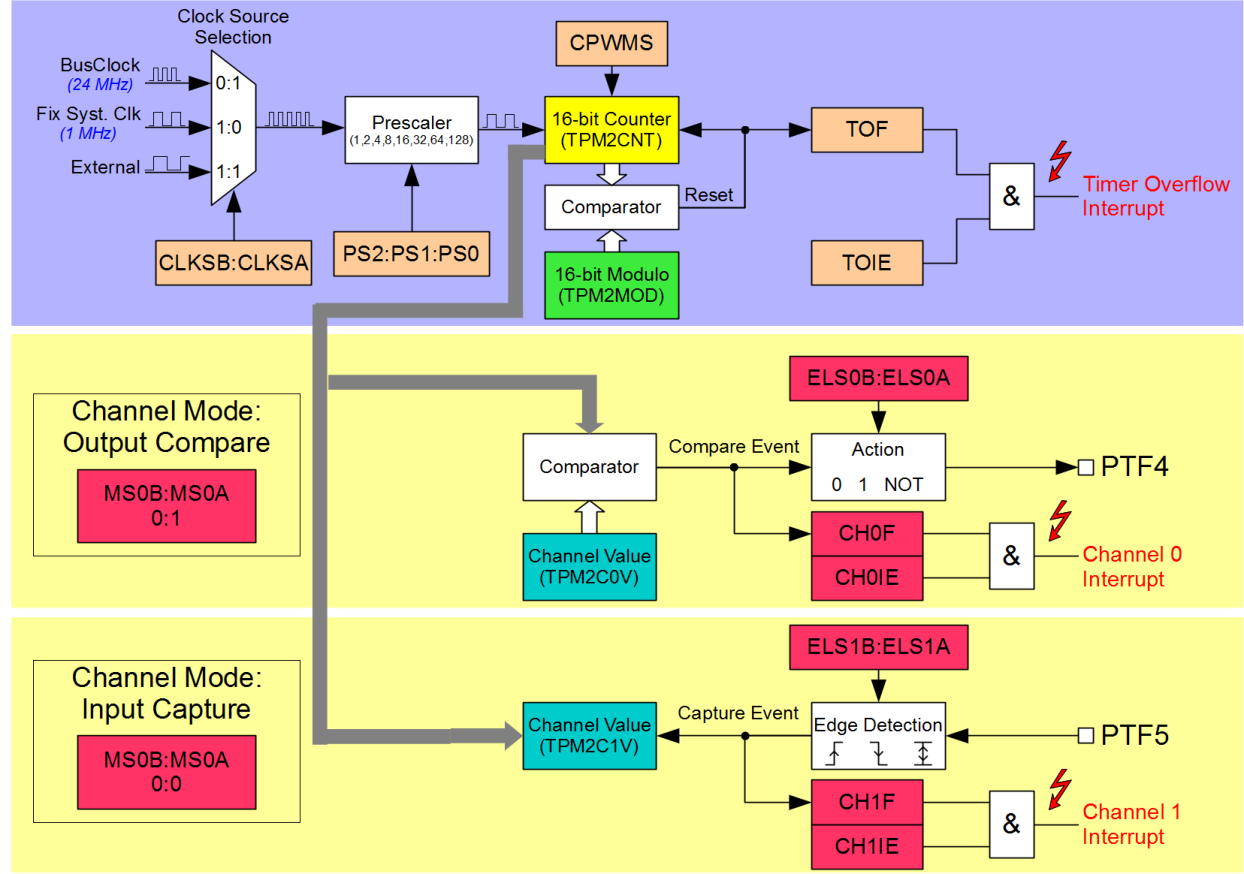
\includegraphics[width=1\textwidth]{../fig/timer.pdf}

	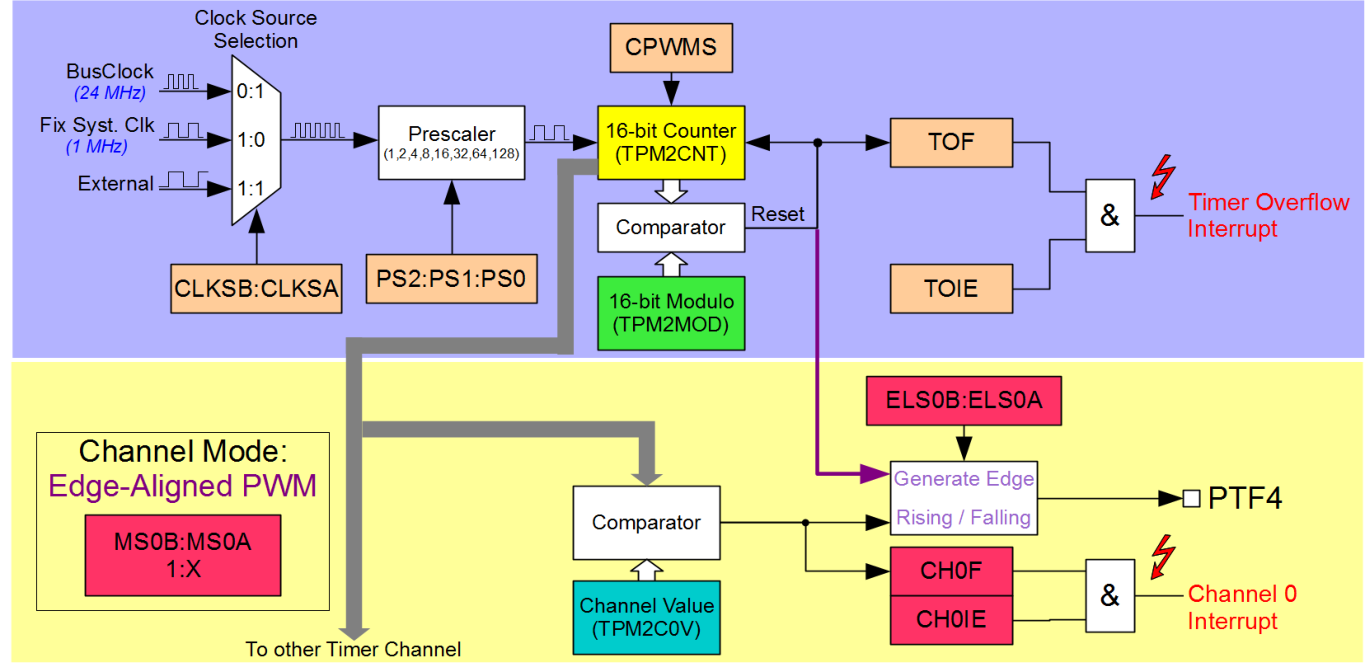
\includegraphics[width=1\textwidth]{../fig/pwm.pdf}
	\caption{Übersicht der Timer-Register}
\end{figure}

\newpage
\subsection{Pitfalls}
\begin{itemize}
	\item Möchte man das Value Register eines Channels setzen, so darf
		der Channel nicht im \emph{Input Capture} Modus sein. In
		diesem Modus wird im Value Register das Snapshot des Counters
		gespeichert bei einem Event.
	\item Arbeitet man mit dem MODULO Wert, so muss dieser auf
		Periodendauer-1 gesetzt werden, da das TOF erst beim
		darauffolgenden Wert des MODULO auslöst.
\end{itemize}

\subsection{Clock \& Prescaler Einstellungen}
\begin{table}[h!]
	\centering
	\begin{tabular}{r r r r}
		Clock-Quelle & Prescaler & Tick & Maximalwert \\
		\hline
		24 MHz & 1 & 0.041667 $\mu$s & 2730.666667 $\mu$s \\ 
		24 MHz & 2 & 0.083333 $\mu$s & 5461.333333 $\mu$s \\ 
		24 MHz & 4 & 0.166667 $\mu$s & 10922.666667 $\mu$s \\ 
		24 MHz & 8 & 0.333333 $\mu$s & 21845.333333 $\mu$s \\ 
		24 MHz & 16 & 0.666667 $\mu$s & 43690.666667 $\mu$s \\ 
		24 MHz & 32 & 1.333333 $\mu$s & 87381.333333 $\mu$s \\ 
		24 MHz & 64 & 2.666667 $\mu$s & 174762.666667 $\mu$s \\ 
		24 MHz & 128 & 5.333333 $\mu$s & 349525.333333 $\mu$s \\ 
		1 MHz & 1 & 1.000000 $\mu$s & 65536.000000 $\mu$s \\ 
		1 MHz & 2 & 2.000000 $\mu$s & 131072.000000 $\mu$s \\ 
		1 MHz & 4 & 4.000000 $\mu$s & 262144.000000 $\mu$s \\ 
		1 MHz & 8 & 8.000000 $\mu$s & 524288.000000 $\mu$s \\ 
		1 MHz & 16 & 16.000000 $\mu$s & 1048576.000000 $\mu$s \\ 
		1 MHz & 32 & 32.000000 $\mu$s & 2097152.000000 $\mu$s \\ 
		1 MHz & 64 & 64.000000 $\mu$s & 4194304.000000 $\mu$s \\ 
		1 MHz & 128 & 128.000000 $\mu$s & 8388608.000000 $\mu$s \\ 
	\end{tabular}
\end{table}

\newpage
\subsection{PWM Varianten}
Ein PWM-Signal kann auf drei verschiedene Arten implmentiert werden
\begin{enumerate}
	\item Timer aufsetzen mit MODULO = Periodendauer, 
		ChannelValue = Implsdauer, Modul-Pin setzen/rücksetzen mit
		CompareEvent Einstellung (ohne ISR)
	\item Timer aufsetzen mit MODULO = Periodendauer,
		ChannelValue = Impulsdauer, beliebigen Pin setzen/rücksetzen
		mit ISR
	\item Timer aufsetzen mit MODULO = DEFAULT, ChannelValue ist
		abwechselnd TimerCounter+Impulszeit und
		TimerCounter+(Periodendauer-Inpulszeit)
\end{enumerate}

\begin{figure}[h!]
	\centering
	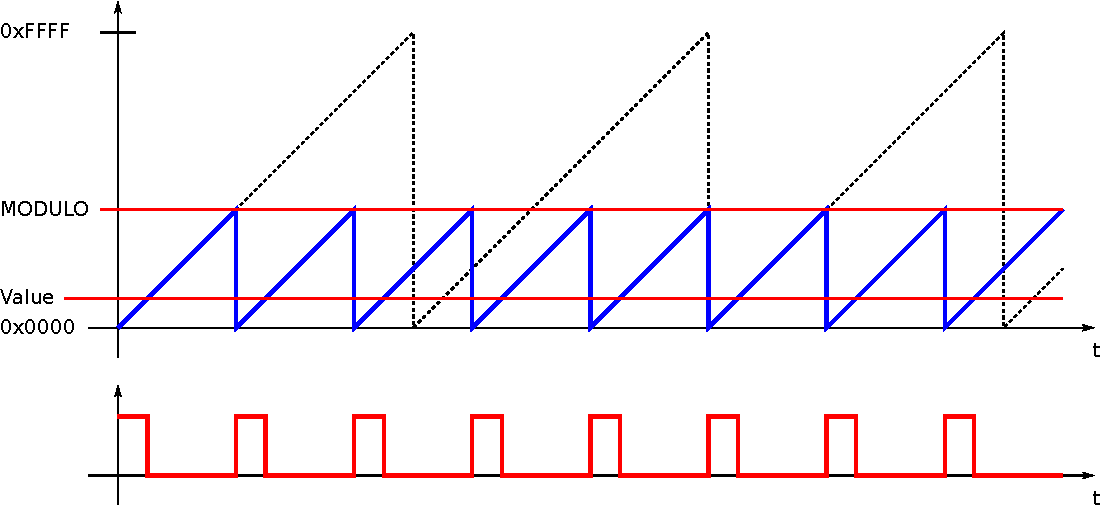
\includegraphics[width=1\textwidth]{../fig/pwm_01.pdf}
	\caption{PWM mit MODULO und ChannelValue}
\end{figure}

\begin{figure}[h!]
	\centering
	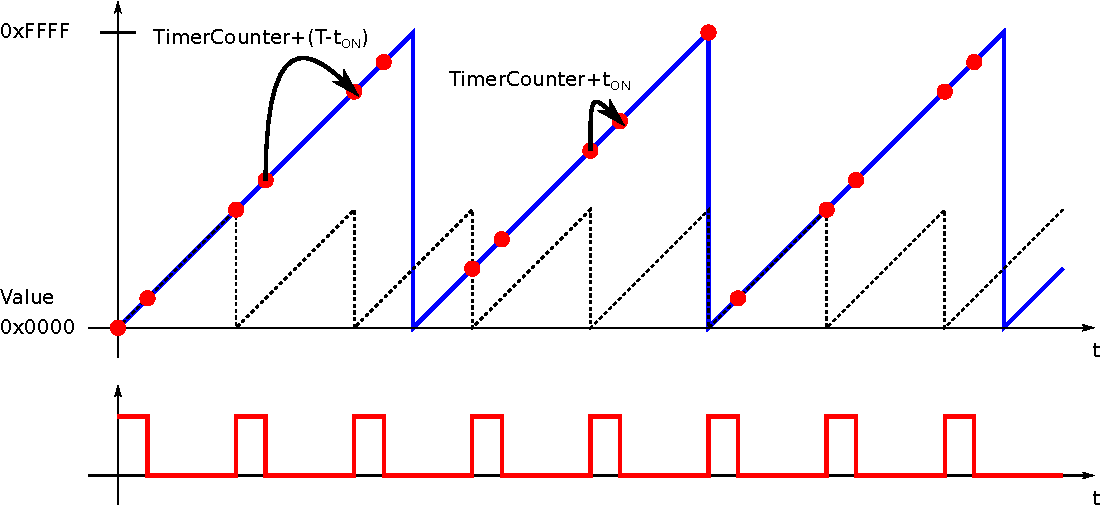
\includegraphics[width=1\textwidth]{../fig/pwm_02.pdf}
	\caption{PWM ohne MODULO}
\end{figure}

\newpage
\subsection{Beispiele}

\subsubsection{Output Compare}
\lstinputlisting[firstline=19, lastline=95, title=main.c]{../src/timer_oc/Sources/main.c}
\lstinputlisting[firstline=60, lastline=60, title=Project.prm]{../src/timer_oc/Project_Settings/Linker_Files/Project.prm}

\newpage
\subsubsection{Input Capture}
\lstinputlisting[title=main.c]{../src/timer_ic_01/Sources/main.c}
\lstinputlisting[firstline=55, lastline=61, title=Project.prm]{../src/timer_ic_01/Project_Settings/Linker_Files/Project.prm}

\begin{comment}
\newpage
\subsubsection{PWM}
\lstinputlisting[firstline=19, lastline=70, title=main.c]{../src/timer_pwm_led/Sources/main.c}
\lstinputlisting[firstline=59, lastline=59, title=Project.prm]{../src/timer_pwm_led/Project_Settings/Linker_Files/Project.prm}
\end{comment}

\newpage
\subsubsection{PWM mit MODULO, VALUE, ohne ISR}
\lstinputlisting[firstline=19, title=PWM - Variante 1]{../src/timer_pwm_var1/Sources/main.c}

\newpage
\subsubsection{PWM mit MODULO, VALUE und ISR}
\lstinputlisting[firstline=19, title=PWM - Variante 2]{../src/mep_timer_pwm_var2/Sources/main.c}

\newpage
\subsubsection{PWM ohne MODULO}
\lstinputlisting[firstline=19, title=PWM - Variante 3]{../src/timer_pwm_var3/Sources/main.c}
